% To compile: pdflatex file.tex
\documentclass{article}
\usepackage{fullpage}
\usepackage{pgffor}
\usepackage{amssymb}
\usepackage{bm}
\usepackage{mathtools}
\usepackage{verbatim}
\usepackage{appendix}
\usepackage{graphicx}
\usepackage{color}
\usepackage{subfig}
\usepackage{url} % for underscore in footnote
\usepackage[UKenglish]{isodate} % for: \today
\cleanlookdateon                % for: \today
%\pagestyle{empty} % Removes page number. Graphs too big.

\def\wl{\par \vspace{\baselineskip}\noindent}
\def\beginmyfig{\begin{figure}[h]\center}
\def\endmyfig{\end{figure}}
\def\ds{\displaystyle}
\def\tu{\textunderscore}
\definecolor{grey}{rgb}{.2,.2,.2}
\definecolor{lgrey}{rgb}{.8,.8,.8}
\def\hline{ \textcolor{lgrey}{\hrulefill} }
\newcommand{\m}[1]{\mathbf{\bm{#1}}} % Serif bold math
\def\ds{\displaystyle}                                                    
\def\inv{^{\raisebox{.2ex}{$\scriptscriptstyle-1$}}}
\def\pm{^{\raisebox{.2ex}{$\scriptscriptstyle\prime$}}}
\def\norm#1{\left\lVert#1\right\rVert}

% \def for THIS ASSIGNMENT!!!%%%%%%%%%%%%%%%%%%%
\usepackage{natbib}

\begin{document}
% my title:
\begin{center}
  {\huge \textbf{Review of the Spatial Dirichlet Process}
    \footnote{\url{https://github.com/luiarthur/bnp_hw/project/bnp_spatialDP}}
  }\\
  \wl
  UCSC AMS 241 Course Project\\
  \noindent\today\\
  Arthur Lui\\
  \hline
\end{center}

This project is a review of the Spatial Dirichlet Process 

\section{Introduction}
In modeling spatial data with replicates, it is possible to cluster replicates

\section{Model}
\[
  \begin{array}{rclcl}
    %\m y_t &|& \m\theta_t,\beta,\tau^2 &\overset{ind.}{\sim}&\text{Normal}_n(\m\theta_t+ \m x_t\beta,
    \m y_t &|& \m\theta_t,\beta,\tau^2 &\overset{ind.}{\sim}&\text{N}_n(\m\theta_t+ \m{1_n}\beta,
    ~\tau^2\m I_n), ~~_{t=1,...,T}\\
    \m\theta_t &|& G^{(n)} &\overset{i.i.d.}{\sim}& G^{(n)}, ~~_{t=1,...,T} \\
    G^{(n)} &|& \alpha, \sigma^2, \phi &\sim& \text{DP}(~\alpha,~\text{N}_n(\m 0_n,\sigma^2H_n(\phi)) ~) \\
    \\
            && \beta, \tau^2 &\sim& \text{N}(m,s^2) \times \text{IGamma}(a_{\tau^2}=2,b_{\tau^2}) \\
            && \alpha &\sim& \text{Gamma}(a_\alpha,b_\alpha) \\
            && \sigma^2 &\sim& \text{IGamma}(b_{\sigma^2}=2,b_{\sigma^2}) \\
            && \phi &\sim& \text{Uniform}(0,b_\phi) \\
  \end{array}
\]
where 
\begin{itemize}
  \item $H_n(\phi)$ is a covariance function, for example, the exponential
    covariance function with decay parameter $\phi$. (i.e.  $(H_n(\phi))_{ij}
    = \exp\left\{-\phi~\norm{s_i-s_j}\right\}$.) \\
  \item $\m y_t(s)$ is the average daily maximum temperature ($^oC$) at location $s$ for replicate $t$.
  %\item $\m y_t$ are the station-measured Ozone levels for the $t^{th}$ replicate.
  %\item $\m x_t$ are a average CMAQ value of the 3 locations nearest to the prediction location for the
  %  $t^{th}$ replicate.
\end{itemize}

\section{Posteriors}
\[\def\arraystretch{1.4}
  \begin{array}{rclcl}
    \beta &|& \m y, \m\theta, \tau^2  &\sim& \text{N}(
      \frac{\tau^2m + s^2\sum_{t=1}^T\sum_{i=1}^n(y_{it}-\theta_{it})}{\tau^2+Tns^2},
      \frac{s^2\tau^2}{\tau^2+Tns^2}) \\
    \tau^2 &|& \m y, \m\theta, \beta  &\sim& \text{IG}(a_{\tau^2}+\frac{nT}{2},
    b_{\tau^2}+\frac{\sum_{t=1}^T (\m\mu_t-\beta \m1_n)'(\m\mu_t-\beta \m1_n)}{2})\\
    %p(\sigma^2 &|& \m\theta_t^*, T^*, \m y, \sigma^2) &\propto& [\sigma^2]\prod_{t=1}^{T^*}
    %  ~\text{N}_n(\m\theta_t^* | \m 0_n,\sigma^2H_n(\phi)) ~)\\
    \sigma^2 &|& \m\theta^*, T^*, \m y, \sigma^2 &\sim& \text{IG}(a_{\sigma^2}+\frac{nT^*}{2},
      %b+\frac{\sum_{t=1}^{T^*}\m\theta^*'Hn^{-1}(\phi)\m\theta^*}{2})\\
    b_{\sigma^2}+\frac{\sum_{t=1}^{T^*}\m\theta_t^{*'} H_n^{-1}(\phi)\m\theta_t^*}{2})\\
    %p(\phi &|& \m\theta_t^*, T^*, \m y, \sigma^2) &\propto& \prod_{t=1}^{T^*} 
    %  ~\text{N}_n(\m\theta_t^* |\m 0_n,\sigma^2H_n(\phi)) ~)\\
    p(\phi &|& \m\theta^*, T^*, \m y, \sigma^2) &\propto& 
    [\phi]|H_n(\phi)|^{-T^*/2} \exp\left(-\frac{\sum_{t=1}^{T^*}\m\theta_t^{*'} H_n^{-1}(\phi)\m\theta_t^*}{2\sigma^2}\right)\\
    \eta &|& \alpha, \m y &\sim& \text{Beta}(\alpha+1,T)\\
    p(\alpha &|& T^*, \m y) &=& (\epsilon)~\gamma(\alpha | a_\alpha+T^*, b_\alpha-\log(\eta)) +\\
             &&&&(1-\epsilon)~\gamma(\alpha | a_\alpha+T^*-1, b_\alpha-\log(\eta))\\
  \end{array}
\]
where $\m\mu_t=\m{y_t -\theta_t} $, $\eta$ is an auxiliary variable introduced
to make the prior for $\alpha$ conjugate, $\gamma$ is the gamma density
function with the mean and rate parameterization, and 
$\epsilon = \ds\frac{a_\alpha +T^* - 1}{ n(b_\alpha-\log(\eta)) + a_\alpha +T^* -1}$.

\section{Posterior for $\m\theta$}
\def\mm{\m{y_t}-\m{1_n}\beta}
\[\def\arraystretch{1.4}
  \begin{array}{rllcl}
    \m\theta_t &|& y_t,\beta,\tau^2,\sigma^2,\phi &\sim& \text{N}_n(\tau^{-2}\m\Lambda(\mm), \m\Lambda)\\
               && q0 &=& |\Lambda|^{1/2} \\
               %&&&& \times \exp\left\{.5\tau^{-2}(\mm)'(\m{I_n}-\tau^{-2}\m\Lambda)(\mm)\right\}\\
               &&&& \times \exp\left\{\frac{(\mm)'(\m{I_n}-\tau^{-2}\m\Lambda)(\mm)}{2\tau^2}\right\}\\
               &&&& \times [(2\pi\tau^2\sigma^2)^{n/2} |\m H_n(\phi)|^{1/2}]^{-1}\\
  \end{array}
\]
where $\m\Lambda = [\tau^{-2}\m I_n + \sigma^{-2} \m H_n^{-1}(\phi)]^{-1}$.


\section{Data}
\beginmyfig 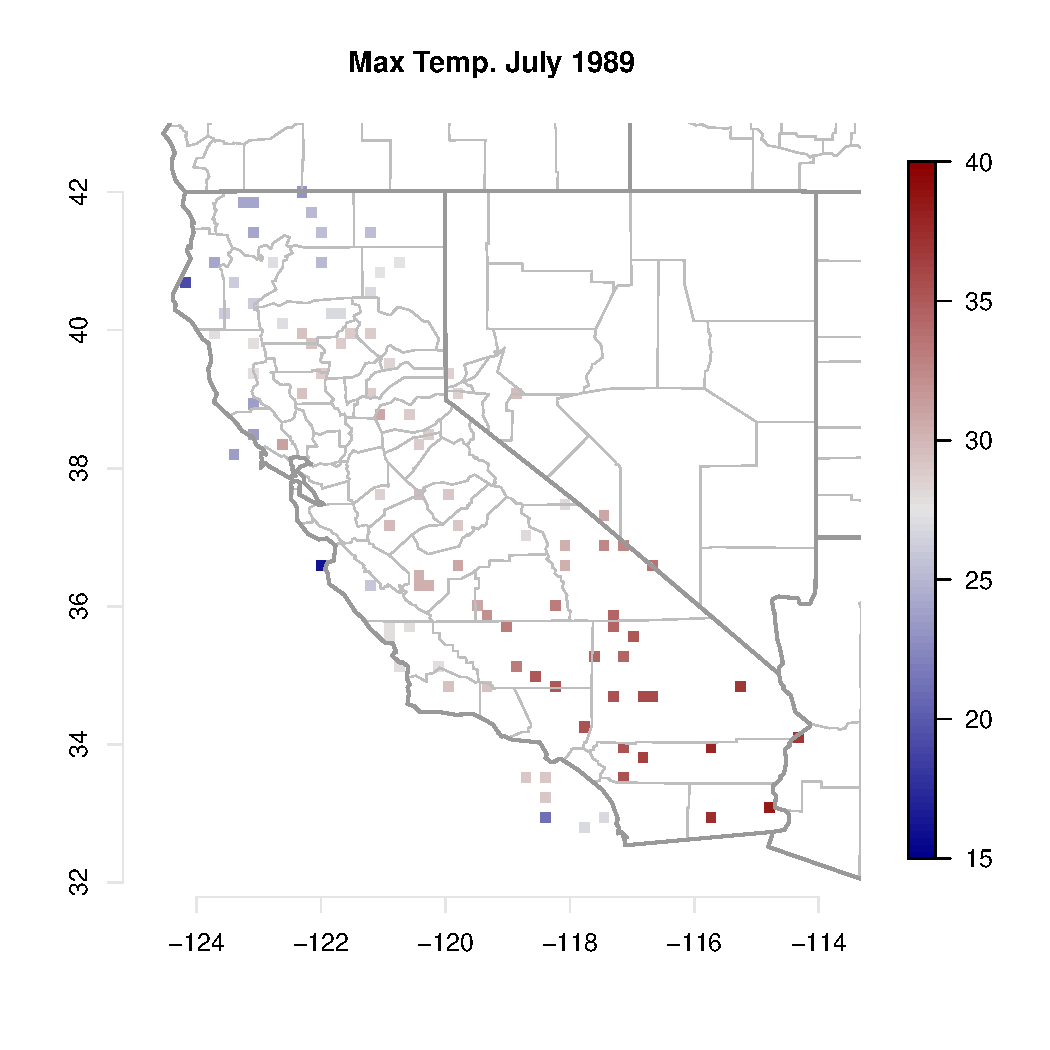
\includegraphics[scale=.5]{../graphs/july1989.pdf} \endmyfig
\section{Results}
\beginmyfig
  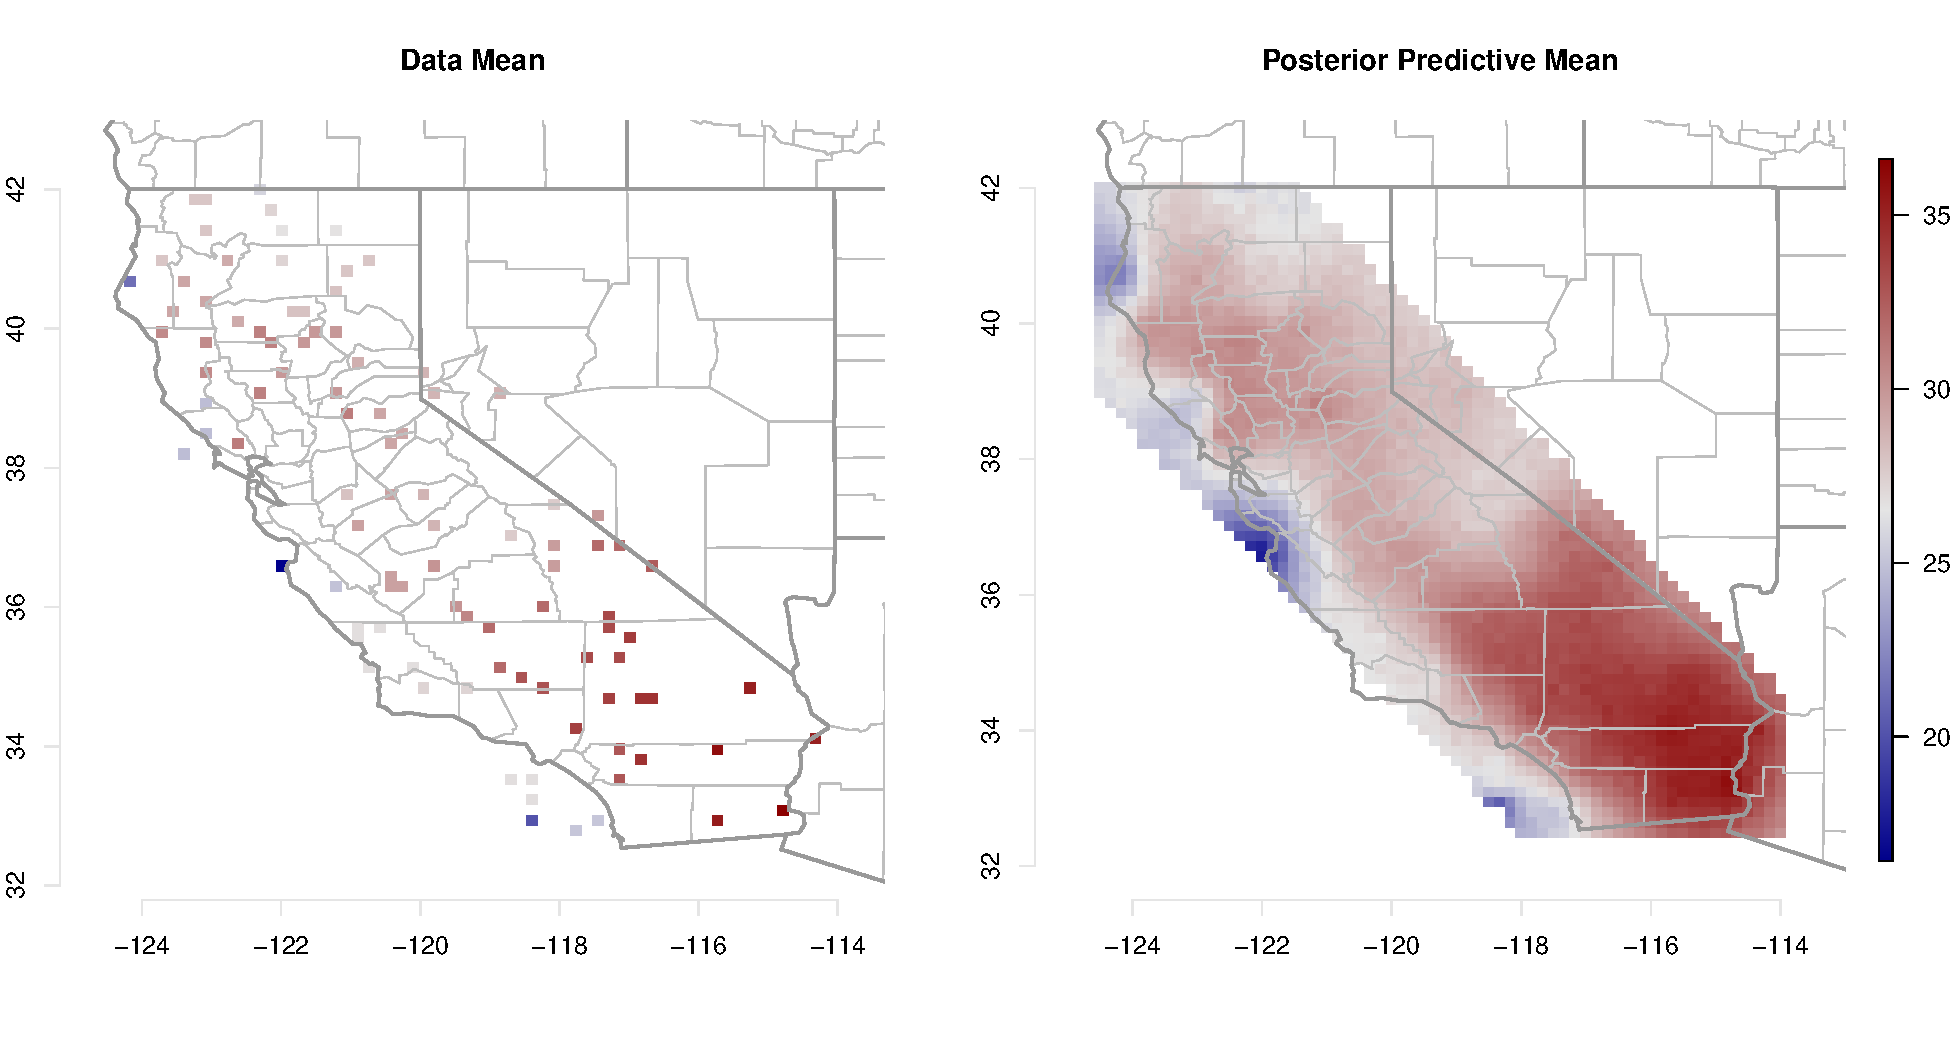
\includegraphics[scale=.35]{../graphs/postpredmean.pdf}
\endmyfig
\beginmyfig
  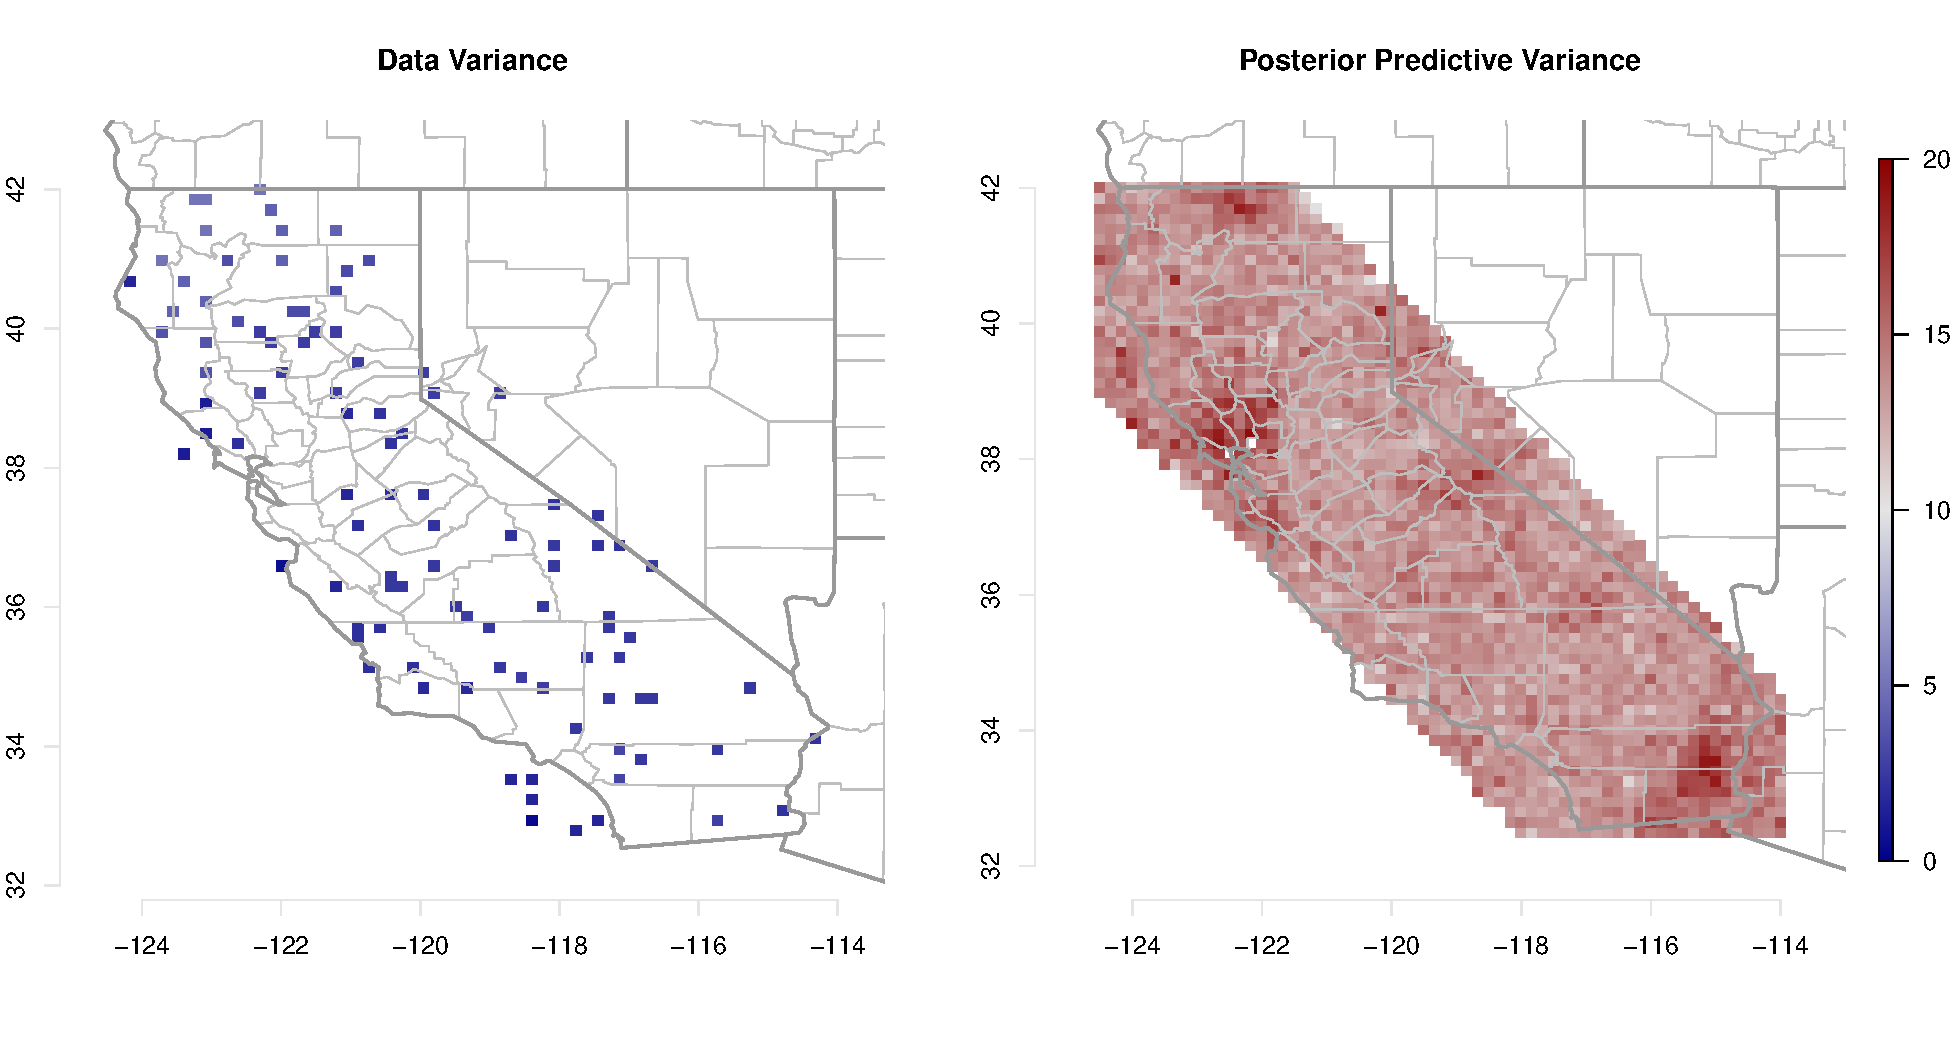
\includegraphics[scale=.35]{../graphs/postpredvar.pdf}
\endmyfig

\cite{sdp}. 
\bibliographystyle{unsrt}
\bibliography{sdp}
\end{document}
